%FOR PDFLATEX USE ONLY
\documentclass[a4paper,12pt]{article}

\usepackage{amssymb,amsmath} %math symbols

\usepackage[margin=2cm]{geometry} %paper geometry

\usepackage[utf8]{inputenc} %allows unicode (including russian) source file
\usepackage[russian]{babel} %docment in russian-style
\usepackage[utf8]{inputenc}
%\usepackage[unicode]{hyperref} %links inside of the text
\usepackage[pdftex]{graphicx} %includegraphics pictures
\usepackage{cmlgc} %bold text

\usepackage{array} %arrays

%\usepackage{wrapfig}
%\usepackage{array}
%\usepackage{lipsum}
%\usepackage{esvect}
%\usepackage{hyperref}

\usepackage{subfig}
%\usepackage{calc}
%\usepackage{pgfplots,tikz,circuitikz}
%\usepackage{tkz-euclide}
\usepackage{booktabs}
\usepackage{multirow}

\begin{document}

\begin{center}
  \LARGE{Работа Д 2.1}\\[0.2cm]
  \LARGE{Определение удельной теплоты парообразования воды}\\[0.2cm]
  \large{Малиновский Владимир}\\[0.2cm]
  \normalsize{\texttt{galqiwi@galqiwi.ru}}
\end{center}

\textbf{Цель работы:} 1) измерение зависимости давления насыщенного пара воды от температуры; 2) вычисление по полученным данным теплоты парообразования с помощью уравнения Клапейрона-Клаузиуса.

\textbf{В работе используются:} шприц на 20 мл и электронный термометр, закреплённые на пластиковой крышке, стеклянная банка, горячая вода, лёд, линейка, водяная баня.

\section*{Описание работы}
В этой работе исследуется зависимость давления насыщенного пара воды от температуры. Для этого используется установка, состоящая из стеклянной банки с водой, в которую вертикально вставлен шприц носиком вниз. Также в крышку банки вставлена термопара для измерения температуры. Методика заключается в том, чтобы залить в эту банку воду при высокой температуре, подождать установления термодинамического равновесия между воздухом в шприце и водой в банке, и измерить зависимость объема смеси газа внутри шарица по мере остывания воды. Этот объем зависит от давления воды, тем самым мы надем зависимость последнего от температуры. Из этой зависимости мы можем найти, например, теплоту преобразования воды, что мы и сделаем.
\section*{Метод обработки данных}
После того, как установится равновесие, внутри шприца будет фиксированное количество воздуха $\nu$. Если при текущей температуре давление жидкости $p$, а атмосферное давление $p_0$, то верно, что
$$p = p_0 - \frac{\nu R T}{V} = p_0 (1 - \frac{T V_0}{T_0 V}),$$
где $V_0$, $T_0$ -- объем и давление, соответствующие комнатным, поскольку при этих условиях давлением жидкости по сравнению с атмосферным можно пренебречь. Таким образом можно получить зависимость давления от температуры.\\
Из этой зависимости можно найти теплоту преобразования через уравнение Клайперона-Клаузиуса
$$p = p_0 \cdot exp\left(\frac{L}{R}\left(\frac{1}{T_{100}} - \frac{1}{T}\right)\right).$$
Построив график $ln(p/p_0)$ от $1/T$, можно найти $L$ -- молярную теплоту параобразования воды.
\newpage
\section*{Ход работы, результаты и обработка}
\subsection*{1}
Соберем установку:
\begin{enumerate}
	\item Проделаем в крышке банки отверстия для шприца и термопары и установим их,
	\item Зальем в банку кипяток и закроем крышкой.
\end{enumerate}
\begin{center}
	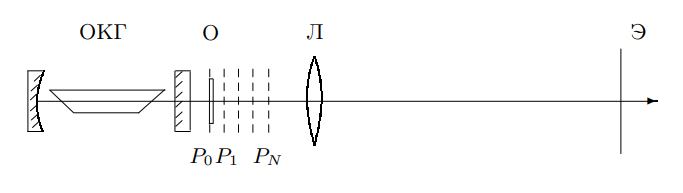
\includegraphics[width=0.80\textwidth]{setup.png}
\end{center}
\subsection*{2}
Проведем измерения:
\begin{enumerate}
	\item Начнем измерение зависимости $V(T)$ в диапазоне $90\,^\circ C-20\,^\circ C$, когда смесь воздуха и водяного пара перестанет выходить из шприца в конце процесса установки равновесия. При низких температурах ($<40\,^\circ C$) добавим лед в воду, чтобы ускорить паление температуры.
	\item Повторим те же измерения при повышении температуры. Для этого банку надо поставить в водяную баню и повторить измерения из прошлого пункта.
\end{enumerate}
У нашей установки был недочет -- мы не двигали термопару так, чтобы она была на середине столба воздуха. Будем надеяться, что, поскольку во время водяной бани мы нагревали банку снизу, а льдом мы охлаждали сверху, из-за конвекции в банке поддерживалась постоянная температура. То, имело ли это место, можно будет увидеть по результатам.\\

\begin{center}
\begin{tabular}{|c|c|c|}\hline
$V,\,\text{дел}$&$T_{\text{нагр}},\,^\circ\text{C}$&$T_{\text{охл}},\,^\circ\text{C}$\\ \hline
$9.0$&$21.0$&$19.0$\\ \hline
$10.0$&$44.0$&$45.0$\\ \hline
$11.0$&$56.0$&$54.0$\\ \hline
$12.0$&$65.0$&$60.0$\\ \hline
$13.0$&$70.0$&$67.0$\\ \hline
$14.0$&$73.0$&$71.0$\\ \hline
$15.0$&$75.0$&$74.0$\\ \hline
$16.0$&$77.0$&$76.0$\\ \hline
$17.0$&$80.0$&$79.0$\\ \hline
$18.0$&$81.0$&$81.0$\\ \hline
$19.0$&$83.0$&$81.0$\\ \hline
$20.0$&$84.0$&$82.0$\\ \hline
$21.0$&$85.0$&$85.0$\\ \hline
$22.0$&$86.0$&$-$\\ \hline
$23.0$&$88.0$&$87.0$\\ \hline
$24.0$&$88.0$&$88.0$\\ \hline
$25.0$&$89.0$&$89.0$\\ \hline
$26.0$&$90.0$&$90.0$\\ \hline
$27.0$&$90.0$&$91.0$\\ \hline
$28.0$&$-$&$92.0$\\ \hline
\end{tabular}
\end{center}
$$\Delta V=0.5\,\,\text{дел},\,\,\Delta T_{\text{нагр}}=0.5\,\,^\circ\text{C},\,\,\Delta T_{\text{охл}}=0.5\,\,^\circ\text{C}.$$
\subsection*{3}
\begin{center}
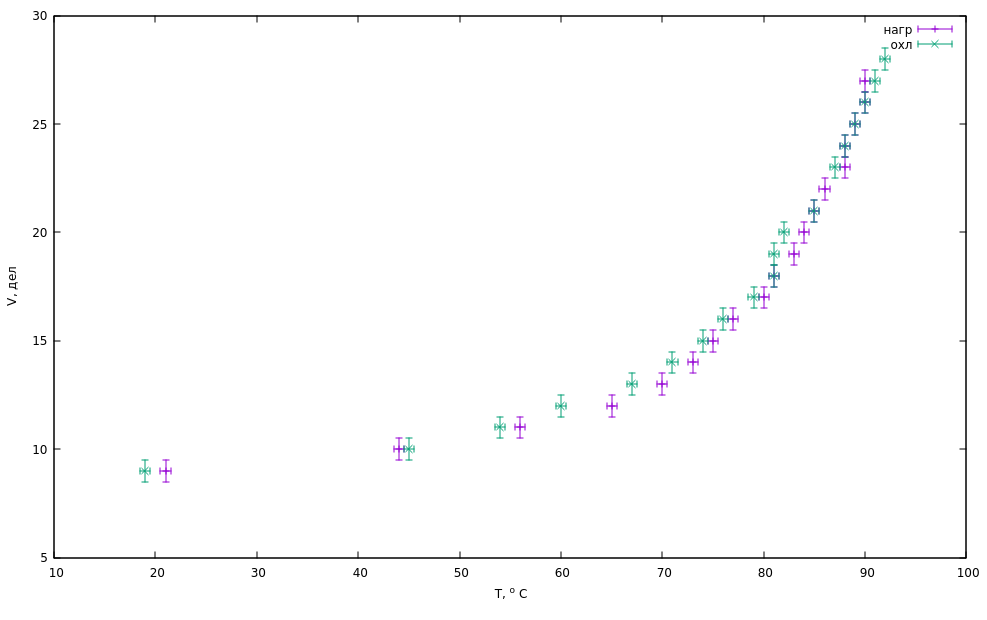
\includegraphics[width=0.80\textwidth]{plot_0.png}
\end{center}
У полученных зависимостей должно быть резкое изменение объема в диапазоне температур между $75\,^\circ C$ и $90\,^\circ C$, и медленный линейный рост при низких ($<35\,^\circ C$) температурах. В наших данных присутствует резкий рост, но, из-за недостаточно маленьких делений на шприце (а они у нас были $2.5\,\text{мм}$), при низких температурах изменение объема почти не наблюдалось. Вообще, из малости следует линейность, но напрямую мы это не проверили.

\subsection*{4, 5}
Из данных можно найти $V_0=(9\pm0.5)\,\text{дел}$ и $T_0=(20\pm1)\,^\circ C$. Зная это, можно найти $p$ по формуле из пункта про обработку данных. Сделаем этот рассчет для точек с температурой $>70\,^\circ C$.

Нагрев:
\begin{center}
\begin{tabular}{|c|c|c|c|c|c|c|c|c|c|c|}\hline
$V,\,\text{дел}$&$T,\,^\circ\text{C}$&$p/p_\text{а}$&$\Delta p/p_\text{а}$
&$ln(p/p_\text{а})$&$\Delta ln(p/p_\text{а})$
&$1000\text{К}/T$&$\Delta 1000\text{К}/T$
\\ \hline
$13.0$&$70.0$&$0.19$&$0.07$&$-1.6$&$0.4$&$2.913$&$0.004$\\ \hline
$14.0$&$73.0$&$0.24$&$0.07$&$-1.4$&$0.2$&$2.888$&$0.004$\\ \hline
$15.0$&$75.0$&$0.29$&$0.06$&$-1.2$&$0.2$&$2.871$&$0.004$\\ \hline
$16.0$&$77.0$&$0.33$&$0.06$&$-1.1$&$0.1$&$2.855$&$0.004$\\ \hline
$17.0$&$80.0$&$0.36$&$0.05$&$-1.01$&$0.15$&$2.830$&$0.004$\\ \hline
$18.0$&$81.0$&$0.40$&$0.05$&$-0.92$&$0.13$&$2.822$&$0.003$\\ \hline
$19.0$&$83.0$&$0.42$&$0.04$&$-0.8$&$0.1$&$2.807$&$0.003$\\ \hline
$20.0$&$84.0$&$0.45$&$0.04$&$-0.7$&$0.1$&$2.799$&$0.003$\\ \hline
$21.0$&$85.0$&$0.48$&$0.04$&$-0.74$&$0.09$&$2.791$&$0.003$\\ \hline
$22.0$&$86.0$&$0.50$&$0.04$&$-0.69$&$0.08$&$2.783$&$0.003$\\ \hline
$23.0$&$88.0$&$0.52$&$0.03$&$-0.65$&$0.07$&$2.768$&$0.003$\\ \hline
$24.0$&$88.0$&$0.54$&$0.03$&$-0.61$&$0.06$&$2.768$&$0.003$\\ \hline
$25.0$&$89.0$&$0.56$&$0.03$&$-0.58$&$0.06$&$2.760$&$0.003$\\ \hline
$26.0$&$90.0$&$0.57$&$0.03$&$-0.55$&$0.05$&$2.753$&$0.003$\\ \hline
$27.0$&$90.0$&$0.59$&$0.03$&$-0.53$&$0.05$&$2.753$&$0.003$\\ \hline
\end{tabular}
\end{center}
$$\Delta V=0.5\,\,\text{дел},\,\,\Delta T=0.5\,\,^\circ\text{C}.$$

Охлаждение:
\begin{center}
\begin{tabular}{|c|c|c|c|c|c|c|c|c|c|c|}\hline
$V,\,\text{дел}$&$T,\,^\circ\text{C}$&$p/p_\text{а}$&$\Delta p/p_\text{а}$
&$ln(p/p_\text{а})$&$\Delta ln(p/p_\text{а})$
&$1000\text{К}/T$&$\Delta 1000\text{К}/T$
\\ \hline
$14.0$&$71.0$&$0.25$&$0.07$&$-1.4$&$0.2$&$2.904$&$0.004$\\ \hline
$15.0$&$74.0$&$0.29$&$0.06$&$-1.2$&$0.2$&$2.879$&$0.004$\\ \hline
$16.0$&$76.0$&$0.33$&$0.06$&$-1.1$&$0.1$&$2.863$&$0.004$\\ \hline
$17.0$&$79.0$&$0.36$&$0.05$&$-1.01$&$0.15$&$2.838$&$0.004$\\ \hline
$18.0$&$81.0$&$0.40$&$0.05$&$-0.92$&$0.13$&$2.822$&$0.003$\\ \hline
$19.0$&$81.0$&$0.43$&$0.04$&$-0.8$&$0.1$&$2.822$&$0.003$\\ \hline
$20.0$&$82.0$&$0.45$&$0.04$&$-0.7$&$0.1$&$2.815$&$0.003$\\ \hline
$21.0$&$85.0$&$0.48$&$0.04$&$-0.74$&$0.09$&$2.791$&$0.003$\\ \hline
$23.0$&$87.0$&$0.52$&$0.03$&$-0.65$&$0.07$&$2.775$&$0.003$\\ \hline
$24.0$&$88.0$&$0.54$&$0.03$&$-0.61$&$0.06$&$2.768$&$0.003$\\ \hline
$25.0$&$89.0$&$0.56$&$0.03$&$-0.58$&$0.06$&$2.760$&$0.003$\\ \hline
$26.0$&$90.0$&$0.57$&$0.03$&$-0.55$&$0.05$&$2.753$&$0.003$\\ \hline
$27.0$&$91.0$&$0.59$&$0.03$&$-0.53$&$0.05$&$2.745$&$0.003$\\ \hline
$28.0$&$92.0$&$0.60$&$0.03$&$-0.51$&$0.05$&$2.737$&$0.003$\\ \hline
\end{tabular}
\end{center}
$$\Delta V=0.5\,\,\text{дел},\,\,\Delta T=0.5\,\,^\circ\text{C}.$$
С помощью этих данных, можно построить зависимость $ln(\frac{p}{p_\text{а}})$ от $1/T$. Коэффициент наклона $A$ у этой линейной зависимости равен $-\frac{L}{R}$. Из этого найдем L:
\begin{center}
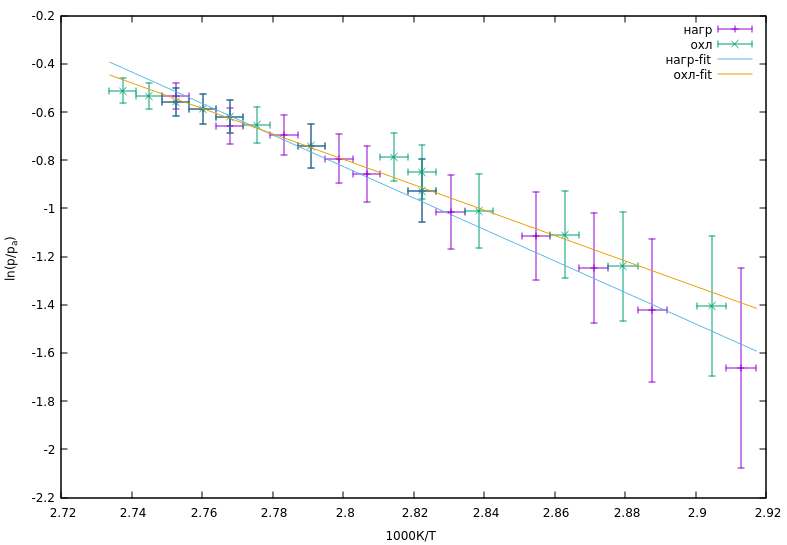
\includegraphics[width=0.95\textwidth]{plot_1.png}
\end{center}
Из графика:
$$A_\text{нагр} = -(6.5\pm0.2)\,\text{КК},\,A_\text{охл} = -(5.3\pm0.2)\,\text{КК}.$$
Если учитывать приборную погрешность:
$$\delta A = \sqrt{\delta A{стат}^2 + \left(\frac{<\Delta ln(p)>}{ln(p)_{max} - ln(p)_{min}}\right)^2 + \left(\frac{<\Delta 1/T>}{(1/T)_{max} - (1/T)_{min}}\right)^2}.$$
$$A_\text{нагр} = -(6.5\pm0.9)\,\text{КК},\,A_\text{охл} = -(5.3\pm0.5)\,\text{КК}.$$
Получаются значения теплоемкости:
$$L_\text{нагр} = (54\pm7)\frac{\text{КДж}}{\text{моль}},\,L_\text{охл} = (44\pm4)\frac{\text{КДж}}{\text{моль}}.$$
Ужельные теплоемкости $r=L/\mu$:
$$L_\text{нагр} = (3.0\pm0.4)\frac{\text{МДж}}{\text{кг}},\,L_\text{охл} = (2.4\pm2)\frac{\text{МДж}}{\text{кг}}.$$
Табличное значение $r=2.3\frac{\text{МДж}}{\text{кг}}$ Значения сходятся (ну, порядок точно сходится, при охлаждении все хорошо, а нагрев отличается на $30\%$).
\section*{Вывод}
Мы научились находить зависимость давления паров жидкости от температуры и находить удельную температуру испарения по этой зависимости через закон Клайперона-Клаузиуса. Полученное значение сходится с табличным не смотря на плохое расположение термопары, хотя, возможно, именно из-за этого при нагреве было отклонение $30\%$. Возможно, также, что это отклонение вызвано тем, что мы слишком быстро нагревали банку, температура бани была заметно выше температуры банки из-за того, что мы выбрали скороводку для того, чтобы ее (баню) сделать, и площадь омывания водой была слишком маленькая.
\end{document}








\lipsum[1-4]
\begin{wrapfigure}{R}{5cm}
\centering
\includegraphics[width=0.20\textwidth]{rd.png}
\caption{1}
\end{wrapfigure}
\lipsum[1-6]


\begin{figure}[h]
\begin{center}$
\begin{array}{cccc}
\includegraphics[width=0.20\textwidth]{rd.png}&
\includegraphics[width=0.20\textwidth]{rd.png}&
\includegraphics[width=0.20\textwidth]{rd.png}&
\includegraphics[width=0.20\textwidth]{rd.png}\\
(1) & (2) & (3) & (4)
\end{array}$
\end{center}
\end{figure}
